There are numerous reasons why CSMA/ECA is more useful when modeled as a decentralized protocol. One being the removal of the Access Point (AP) as a single point of failure. Also, AP Beacons are no longer used as a control measure to estimate the number of contenders in the network, which in turn reduces the overall convergence time.

% In order to model the protocol, it is treated a Decentralized Constraint Satisfaction (DCS) problem~\cite{DCSP, DCSP-E2CA} using the ACK as the only feedback information that identifies a successful transmission.

If $\eta > C$ and under saturation (all contenders have something to transmit, all the time), $\eta - C$ contenders are forced to choose a random backoff, given that there are no unpicked slots available for transmission. This in turn provokes collisions on the $C$ remaining nodes that picked a slot using a deterministic backoff~\cite{CSMA_ECA}. 

CSMA/E2CA manages this issue forcing the nodes to \emph{stick} to a deterministic backoff. That is, the contenders will choose a deterministic backoff two times after a successful transmission. If two consecutive collisions occur, then the contender will be forced to double its contention window (by incrementing the backoff stage, $m$ in Eq.~\ref{eq:backoff_stage}) and to pick a random backoff. This results in a faster convergence to a collision-free state, but at the same time reduces the fairness of the protocol given that some contenders may have to wait more than others to access the channel.

\begin{equation} \label{eq:backoff_stage}
	W = 2^{m}CW_{min},\ m\in[0,...,5]
\end{equation}

\subsection{Ensuring fairness}
Under CSMA/E2CA, nodes may have different contention windows ($W$ in Eq.~\ref{eq:backoff_stage}), this means that some arbitrary contenders have to wait more than others in order to access the channel; compromising the fairness of the protocol. To leverage this issue, nodes are set to transmit $2^{m}$ packets every time their backoff counter expires. That is, if a contender doubled its contention window, then it will also double the packets that are going to be transmitted on the next opportunity. This fairness mechanism for CSMA/E2CA is called Fair Share from here on.

\begin{figure}[htbp]
  \centering
  \includegraphics[width=0.7\linewidth, angle = -90]{figures/throughput/CSMA-E2CA_w_fairShare.eps}
  \caption{Throughput and Jain's Fairness Index when implementing Fair Share in CSMA/E2CA
  \label{fig:fairShare}}
\end{figure}

In Figure~\ref{fig:fairShare} it is appreciated through the estimation of the Jain's Fairness Index~\cite{JFI} that by implementing Fair Share every contender receives almost the same service time, therefore the system is considered fair.